% questions.tex —— 2013 年·四川卷·文科 · 题目内容片段（无答案）
% 由 tools/generate_projects.py 依来源总账自 2013/2013_数学真题_四川文_试题.md 生成，勿手改（改源 MD 后重跑）
\gkpart{一、选择题}
\begin{question}
\gkti{1}设集合 $A=\{1,2,3\}$，集合 $B=\{-2,2\}$，则 $A\cap B=$\mbox{（　　）}
（A）$\varnothing$；（B）$\{2\}$；（C）$\{-2,2\}$；（D）$\{-2,1,2,3\}$。
\Needspace{0.4\textheight}
\end{question}
\begin{question}
\gkti{2}一个几何体的三视图如图所示，则该几何体可以是\mbox{（　　）}
\nopagebreak[4]
\begin{center}% 2013 四川卷文科第 2 题：几何体的三视图（正、侧视图为等腰梯形，俯视图为同心圆）。
\begin{tikzpicture}[font=\footnotesize, line width=0.45pt, scale=1]
  % 正视图：梯形
  \draw (0.35,0) -- (2.95,0) -- (2.20,1.55) -- (1.10,1.55) -- cycle;
  \node[below] at (1.65,-0.16) {正视图};
  % 侧视图：梯形
  \draw (4.55,0) -- (7.15,0) -- (6.40,1.55) -- (5.30,1.55) -- cycle;
  \node[below] at (5.85,-0.16) {侧视图};
  % 俯视图：同心圆
  \draw (1.65,-1.55) circle (0.90);
  \draw (1.65,-1.55) circle (0.46);
  \node[below] at (1.65,-2.62) {俯视图};
\end{tikzpicture}
\end{center}
\nopagebreak[4]
（A）棱柱；（B）棱台；（C）圆柱；（D）圆台。
\Needspace{0.4\textheight}
\end{question}
\begin{question}
\gkti{3}如图，在复平面内，点 $A$ 表示复数 $z$，则图中表示 $z$ 的共轭复数的点是\mbox{（　　）}
\nopagebreak[4]
\begin{center}% 2013 四川卷文科第 3 题：复平面内点 A 表示复数 z，B、C、D 为其余候选点。
\begin{tikzpicture}[font=\footnotesize, line width=0.45pt, >=Stealth, scale=1]
  \draw[->] (-2.8,0) -- (2.7,0) node[right] {$x$};
  \draw[->] (0,-1.95) -- (0,1.95) node[above] {$y$};
  \node[below left] at (0.06,0) {$O$};
  \fill (-1.85,1.15) circle (1.4pt);
  \node[above left] at (-1.85,1.15) {$A$};
  \fill (-1.85,-1.15) circle (1.4pt);
  \node[below left] at (-1.85,-1.15) {$B$};
  \fill (1.55,-1.15) circle (1.4pt);
  \node[below right] at (1.55,-1.15) {$C$};
  \fill (1.55,1.15) circle (1.4pt);
  \node[above right] at (1.55,1.15) {$D$};
\end{tikzpicture}
\end{center}
\nopagebreak[4]
（A）$A$；（B）$B$；（C）$C$；（D）$D$。
\end{question}
\begin{question}
\gkti{4}设 $x\in\mathbf Z$，集合 $A$ 是奇数集，集合 $B$ 是偶数集。若命题 $p$：$\forall x\in A$，$2x\in B$，则\mbox{（　　）}
（A）$\neg p$：$\exists x\in A$，$2x\in B$；（B）$\neg p$：$\exists x\notin A$，$2x\in B$；（C）$\neg p$：$\exists x\in A$，$2x\notin B$；（D）$\neg p$：$\forall x\notin A$，$2x\notin B$。
\end{question}
\begin{question}
\gkti{5}抛物线 $y^2=8x$ 的焦点到直线 $x-\sqrt3y=0$ 的距离是\mbox{（　　）}
（A）$2\sqrt3$；（B）$2$；（C）$\sqrt3$；（D）$1$。
\Needspace{0.4\textheight}
\end{question}
\begin{question}
\gkti{6}函数 $f(x)=2\sin(\omega x+\varphi)$（$\omega>0$，$-\dfrac\pi2<\varphi<\dfrac\pi2$）的部分图象如图所示，则 $\omega$，$\varphi$ 的值分别是\mbox{（　　）}
\nopagebreak[4]
\begin{center}% 2013 四川卷文科第 6 题：$f(x)=2\sin(\omega x+\varphi)$ 的部分图象。
\begin{tikzpicture}[font=\footnotesize, line width=0.45pt, >=Stealth,
  x=2.15cm, y=0.86cm]
  \draw[->] (-0.42,0) -- (3.85,0) node[below] {$x$};
  \draw[->] (0,-2.62) -- (0,2.72) node[right] {$y$};
  \node[below left] at (0,0) {$O$};
  % 峰值与谷值的辅助虚线
  \draw[dashed] (0,2) -- ({5*pi/12},2) -- ({5*pi/12},0);
  \draw[dashed] (0,-2) -- ({11*pi/12},-2) -- ({11*pi/12},0);
  % 图象
  \draw[domain=0:3.52, samples=240, smooth]
    plot (\x, {2*sin(deg(2*\x-pi/3))});
  \node[left] at (0,2) {$2$};
  \node[left] at (0,-2) {$-2$};
  \node[below] at ({5*pi/12},-0.12) {$\dfrac{5\pi}{12}$};
  \node[above left] at ({11*pi/12},0.10) {$\dfrac{11\pi}{12}$};
\end{tikzpicture}
\end{center}
\nopagebreak[4]
（A）$2$，$-\dfrac\pi3$；（B）$2$，$-\dfrac\pi6$；（C）$4$，$-\dfrac\pi6$；（D）$4$，$\dfrac\pi3$。
\Needspace{0.4\textheight}
\end{question}
\begin{question}
\gkti{7}某学校随机抽取 $20$ 个班，调查各班中有网上购物经历的人数，所得数据的茎叶图如图所示，以组距为 $5$ 将数据分组成 $[0,5)$，$[5,10)$，$\cdots$，$[30,35)$，$[35,40]$ 时，所作的频率分布直方图是\mbox{（　　）}
\nopagebreak[4]
\begin{center}% 2013 四川卷文科第 7 题：20 个班中有网上购物经历人数的茎叶图。
\begin{tikzpicture}[font=\small, line width=0.45pt, x=1cm, y=1cm]
  % 茎叶图的分隔线
  \draw (-0.55,0.52) -- (5.00,0.52);
  \draw (0.24,0.52) -- (0.24,-2.62);
  % 茎
  \foreach \s/\y in {0/0, 1/-0.78, 2/-1.56, 3/-2.34} {
    \node[anchor=east] at (-0.06,\y) {$\s$};
  }
  % 叶（自左向右按原图由大到小排列）
  \foreach \v [count=\i from 1] in {7,3} {
    \node at ({0.60+(\i-1)*0.60},0) {$\v$};
  }
  \foreach \v [count=\i from 1] in {7,6,4,4,3,0} {
    \node at ({0.60+(\i-1)*0.60},-0.78) {$\v$};
  }
  \foreach \v [count=\i from 1] in {7,5,5,4,3,2,0} {
    \node at ({0.60+(\i-1)*0.60},-1.56) {$\v$};
  }
  \foreach \v [count=\i from 1] in {8,5,4,3,0} {
    \node at ({0.60+(\i-1)*0.60},-2.34) {$\v$};
  }
\end{tikzpicture}
\end{center}
\nopagebreak[4]
\nopagebreak[4]
\begin{center}% 2013 四川卷文科第 7 题：四个频率分布直方图选项 (A)—(D)。
% 组距 5 时 频率/组距 = 频数/100：(A) 频数 1,1,4,2,4,3,3,2（正确），
% (B) 1,2,3,3,5,2,3,1；(C)(D) 误用组距 10。
\newcommand{\freqpanel}[5]{%
  \begin{scope}[shift={#1}, x=0.142cm, y=58cm]
    \draw[->] (0,0) -- (44,0) node[above left, inner sep=3pt] {\small 人数};
    \draw[->] (0,0) -- (0,{#2*1.36});
    \node[above, inner sep=1pt] at (0,{#2*1.42})
      {$\dfrac{\text{频率}}{\text{组距}}$};
    % 纵轴刻度
    \foreach \v in {#4} {
      \draw (-0.9,\v) -- (0,\v);
      \node[left, inner sep=1.5pt] at (-1.0,\v) {\v};
    }
    % 横轴刻度
    \foreach \t in {#3} {
      \draw (\t,-0.0016) -- (\t,0.0016);
      \node[below, inner sep=1.5pt] at (\t,-0.0019) {\t};
    }
    % 柱形
    \foreach \h [count=\i from 1] in {#5} {
      \draw ({(\i-1)*\barw},0) rectangle ({\i*\barw},\h);
    }
  \end{scope}%
}
\begin{tikzpicture}[font=\scriptsize, line width=0.45pt, >=Stealth]
  \def\barw{5}
  \freqpanel{(0,0)}{0.04}{0,5,...,40}{0.01,0.02,0.03,0.04}
    {0.01,0.01,0.04,0.02,0.04,0.03,0.03,0.02}
  \node at (-0.55,-1.15) {(A)};
  \freqpanel{(7.4,0)}{0.05}{0,5,...,40}{0.01,0.02,0.03,0.04,0.05}
    {0.01,0.02,0.03,0.03,0.05,0.02,0.03,0.01}
  \node at (6.85,-1.15) {(B)};
  \def\barw{10}
  \freqpanel{(0,-5.6)}{0.04}{0,10,20,30,40}{0.01,0.02,0.03,0.04}
    {0.01,0.03,0.035,0.025}
  \node at (-0.55,-6.75) {(C)};
  \freqpanel{(7.4,-5.6)}{0.04}{0,10,20,30,40}{0.01,0.02,0.03,0.04}
    {0.015,0.03,0.035,0.02}
  \node at (6.85,-6.75) {(D)};
\end{tikzpicture}
\end{center}
\nopagebreak[4]
\end{question}
\begin{question}
\gkti{8}若变量 $x$，$y$ 满足约束条件
\nopagebreak[4]
\[\begin{cases}x+y\leqslant8,\\[2pt] 2y-x\leqslant4,\\[2pt] x\geqslant0,\\[2pt] y\geqslant0,\end{cases}\]
且 $z=5y-x$ 的最大值为 $a$，最小值为 $b$，则 $a-b$ 的值是\mbox{（　　）}
（A）$48$；（B）$30$；（C）$24$；（D）$16$。
\end{question}
\begin{question}
\gkti{9}从椭圆 $\dfrac{x^2}{a^2}+\dfrac{y^2}{b^2}=1$（$a>b>0$）上一点 $P$ 向 $x$ 轴作垂线，垂足恰为左焦点 $F_1$，$A$ 是椭圆与 $x$ 轴正半轴的交点，$B$ 是椭圆与 $y$ 轴正半轴的交点，且 $AB\parallel OP$（$O$ 是坐标原点），则该椭圆的离心率是\mbox{（　　）}
（A）$\dfrac{\sqrt2}{4}$；（B）$\dfrac12$；（C）$\dfrac{\sqrt2}{2}$；（D）$\dfrac{\sqrt3}{2}$。
\end{question}
\begin{question}
\gkti{10}设函数 $f(x)=\sqrt{\mathrm e^x+x-a}$（$a\in\mathbf R$，$\mathrm e$ 为自然对数的底数）。若存在 $b\in[0,1]$ 使 $f(f(b))=b$ 成立，则 $a$ 的取值范围是\mbox{（　　）}
（A）$[1,\mathrm e]$；（B）$[1,1+\mathrm e]$；（C）$[\mathrm e,1+\mathrm e]$；（D）$[0,1]$。
\end{question}
\gkpart{二、填空题}
\begin{question}
\gkti{11}$\lg\sqrt5+\lg\sqrt{20}$ 的值是\gkblank{}。
\Needspace{0.4\textheight}
\end{question}
\begin{question}
\gkti{12}在平行四边形 $ABCD$ 中，对角线 $AC$ 与 $BD$ 交于点 $O$，$\overrightarrow{AB}+\overrightarrow{AD}=\lambda\overrightarrow{AO}$，则 $\lambda=$\gkblank{}。
\nopagebreak[4]
\begin{center}% 2013 四川卷文科第 12 题：平行四边形 ABCD，对角线 AC、BD 交于点 O。
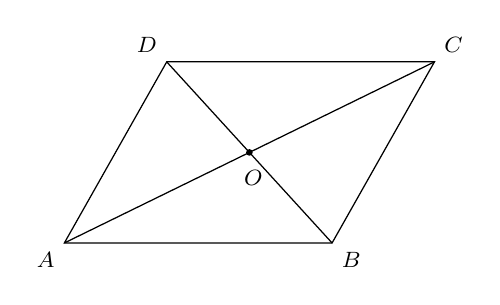
\begin{tikzpicture}[font=\footnotesize, line width=0.45pt, scale=1]
  \coordinate (A) at (0,0);
  \coordinate (B) at (3.4,0);
  \coordinate (C) at (4.7,2.3);
  \coordinate (D) at (1.3,2.3);
  \coordinate (O) at (2.35,1.15);
  \draw (A) -- (B) -- (C) -- (D) -- cycle;
  \draw (A) -- (C);
  \draw (B) -- (D);
  \fill (O) circle (1.2pt);
  \node[below left]  at (A) {$A$};
  \node[below right] at (B) {$B$};
  \node[above right] at (C) {$C$};
  \node[above left]  at (D) {$D$};
  \node[below]       at (2.40,1.05) {$O$};
\end{tikzpicture}
\end{center}
\nopagebreak[4]
\end{question}
\begin{question}
\gkti{13}已知函数 $f(x)=4x+\dfrac ax$（$x>0$，$a>0$）在 $x=3$ 时取得最小值，则 $a=$\gkblank{}。
\end{question}
\begin{question}
\gkti{14}设 $\sin2\alpha=-\sin\alpha$，$\alpha\in\left(\dfrac\pi2,\pi\right)$，则 $\tan2\alpha$ 的值是\gkblank{}。
\end{question}
\begin{question}
\gkti{15}在平面直角坐标系内，到点 $A(1,2)$，$B(1,5)$，$C(3,6)$，$D(7,-1)$ 的距离之和最小的点的坐标是\gkblank{}。
\end{question}
\gkpart{三、解答题}
\begin{question}
\gkti{16}在等比数列 $\{a_n\}$ 中，$a_2-a_1=2$，且 $2a_2$ 为 $3a_1$ 和 $a_3$ 的等差中项，求数列 $\{a_n\}$ 的首项、公比及前 $n$ 项和。
\end{question}
\begin{question}
\gkti{17}在 $\triangle ABC$ 中，角 $A$，$B$，$C$ 的对边分别为 $a$，$b$，$c$，且 $\cos(A-B)\cos B-\sin(A-B)\sin(A+C)=-\dfrac35$。
（1） 求 $\sin A$ 的值；
（2） 若 $a=4\sqrt2$，$b=5$，求向量 $\overrightarrow{BA}$ 在 $\overrightarrow{BC}$ 方向上的投影。
\Needspace{0.4\textheight}
\end{question}
\begin{question}
\gkti{18}某算法的程序框图如图所示，其中输入的变量 $x$ 在 $1,2,3,\cdots,24$ 这 $24$ 个整数中等可能随机产生。
\nopagebreak[4]
\begin{center}% 2013 四川卷文科第 18 题：输出 y 的值的程序框图。
\begin{tikzpicture}[font=\footnotesize, >=Stealth, line width=0.45pt,
  node distance=4.6mm,
  term/.style={draw, rounded corners=5pt, minimum height=1.8em, inner xsep=8pt},
  io/.style={draw, trapezium, trapezium left angle=72, trapezium right angle=108,
             minimum height=1.8em, inner xsep=7pt},
  box/.style={draw, minimum height=1.8em, inner xsep=6pt},
  dec/.style={draw, diamond, aspect=2.4, inner sep=1pt}]
  \node[term] (start) {开始};
  \node[io, below=5mm of start] (input) {输入 $x$};
  \node[dec, below=6mm of input] (even) {$x$ 为偶数?};
  \node[box, right=9mm of even] (y1) {$y=1$};
  \node[dec, below=9mm of even] (div) {$x$ 能被 3 整除?};
  \node[box, left=9mm of div] (y2) {$y=2$};
  \node[box, below=6mm of div] (y3) {$y=3$};
  \node[io, below=15mm of y3] (output) {输出 $y$};
  \node[term, below=5mm of output] (end) {结束};
  \draw[->] (start) -- (input);
  \draw[->] (input) -- (even);
  \draw[->] (even) -- node[above] {否} (y1);
  \draw[->] (even) -- node[right] {是} (div);
  \draw[->] (div) -- node[above] {否} (y2);
  \draw[->] (div) -- node[right] {是} (y3);
  \draw[->] (y1.south) |- (output.east);
  \draw[->] (y2.south) |- (output.west);
  \draw[->] (y3) -- (output);
  \draw[->] (output) -- (end);
\end{tikzpicture}
\end{center}
\nopagebreak[4]
（1） 分别求出按程序框图正确编程运行时输出 $y$ 的值为 $i$ 的概率 $P_i$（$i=1,2,3$）；
（2） 甲、乙两同学依据自己对程序框图的理解，各自编写程序重复运行 $n$ 次后，统计记录了输出 $y$ 的值为 $i$（$i=1,2,3$）的频数。以下是甲、乙所作频数统计表的部分数据。
甲的频数统计表（部分）：
\begin{center}
\begin{tabular}{llll}
\toprule
运行次数 $n$ & 输出 $y$ 为 $1$ 的频数 & 输出 $y$ 为 $2$ 的频数 & 输出 $y$ 为 $3$ 的频数 \\
\midrule
$30$ & $14$ & $6$ & $10$ \\
$\cdots$ & $\cdots$ & $\cdots$ & $\cdots$ \\
$2100$ & $1027$ & $376$ & $697$ \\
\bottomrule
\end{tabular}
\end{center}
乙的频数统计表（部分）：
\begin{center}
\begin{tabular}{llll}
\toprule
运行次数 $n$ & 输出 $y$ 为 $1$ 的频数 & 输出 $y$ 为 $2$ 的频数 & 输出 $y$ 为 $3$ 的频数 \\
\midrule
$30$ & $12$ & $11$ & $7$ \\
$\cdots$ & $\cdots$ & $\cdots$ & $\cdots$ \\
$2100$ & $1051$ & $696$ & $353$ \\
\bottomrule
\end{tabular}
\end{center}
当 $n=2100$ 时，根据表中的数据，分别写出甲、乙所编程序各自输出 $y$ 的值为 $i$（$i=1,2,3$）的频率（用分数表示），并判断两位同学中哪一位所编写程序符合算法要求的可能性较大。
\Needspace{0.4\textheight}
\end{question}
\begin{question}
\gkti{19}如图，在三棱柱 $ABC-A_1B_1C_1$ 中，侧棱 $AA_1\perp$ 底面 $ABC$，$AB=AC=2AA_1=2$，$\angle BAC=120^\circ$，$D$，$D_1$ 分别是线段 $BC$，$B_1C_1$ 的中点，点 $P$ 是线段 $AD$ 上异于端点的点。
\nopagebreak[4]
\begin{center}% 2013 四川卷文科第 19 题：三棱柱 ABC-A1B1C1，D、D1 分别为 BC、B1C1 的中点，P 在 AD 上。
\begin{tikzpicture}[font=\footnotesize, line width=0.45pt, scale=1]
  \coordinate (C)  at (0.80,3.40);
  \coordinate (A)  at (2.60,2.00);
  \coordinate (B)  at (5.60,2.00);
  \coordinate (C1) at (0.80,1.60);
  \coordinate (A1) at (2.60,0.20);
  \coordinate (B1) at (5.60,0.20);
  \coordinate (D)  at (3.20,2.70);
  \coordinate (D1) at (3.20,0.90);
  \coordinate (P)  at (2.87,2.315);
  % 顶面三角形
  \draw (A) -- (B) -- (C) -- cycle;
  % 可见的侧棱与底面棱
  \draw (A) -- (A1);
  \draw (B) -- (B1);
  \draw (C) -- (C1);
  \draw (A1) -- (B1);
  % 平面 A1BC 的辅助线
  \draw (A1) -- (C);
  \draw (A1) -- (B);
  % 被遮挡的棱
  \draw[dashed] (C1) -- (A1);
  \draw[dashed] (C1) -- (B1);
  \draw[dashed] (D)  -- (D1);
  % 点与标注
  \fill (P) circle (1.4pt);
  \node[above left]  at (C)  {$C$};
  \node[below left]  at (2.48,1.86) {$A$};
  \node[right]       at (B)  {$B$};
  \node[left=3pt]    at (C1) {$C_1$};
  \node[below left]  at (A1) {$A_1$};
  \node[below right=1pt] at (B1) {$B_1$};
  \node[above left]  at (D)  {$D$};
  \node[right]       at ($(D1)+(0.10,0)$) {$D_1$};
  \node[left]        at (P)  {$P$};
\end{tikzpicture}
\end{center}
\nopagebreak[4]
（1） 在平面 $ABC$ 内，试作出过点 $P$ 与平面 $A_1BC$ 平行的直线 $l$，请说明理由，并证明直线 $l\perp$ 平面 $ADD_1A_1$；
（2） 设（1）中的直线 $l$ 交 $AC$ 于点 $Q$，求三棱锥 $A_1-QC_1D$ 的体积。
（锥体体积公式：$V=\dfrac13Sh$，其中 $S$ 为底面面积，$h$ 为高）
\end{question}
\begin{question}
\gkti{20}已知圆 $C$ 的方程为 $x^2+(y-4)^2=4$，点 $O$ 是坐标原点，直线 $l$：$y=kx$ 与圆 $C$ 交于 $M$，$N$ 两点。
（1） 求 $k$ 的取值范围；
（2） 设 $Q(m,n)$ 是线段 $MN$ 上的点，且 $\dfrac2{|OQ|^2}=\dfrac1{|OM|^2}+\dfrac1{|ON|^2}$，请将 $n$ 表示为 $m$ 的函数。
\end{question}
\begin{question}
\gkti{21}已知函数 $f(x)=\begin{cases}x^2+2x+a,&x<0,\\[2pt] \ln x,&x>0,\end{cases}$ 其中 $a$ 是实数。设 $A(x_1,f(x_1))$，$B(x_2,f(x_2))$ 为该函数图象上的两点，且 $x_1<x_2$。
（1） 指出函数 $f(x)$ 的单调区间；
（2） 若函数 $f(x)$ 的图象在点 $A$，$B$ 处的切线互相垂直，且 $x_2<0$，证明：$x_2-x_1\geqslant1$；
（3） 若函数 $f(x)$ 的图象在点 $A$，$B$ 处的切线重合，求 $a$ 的取值范围。

\end{question}